%!TEX TS-program = xelatex
%!TEX encoding = UTF-8 Unicode
%times,

\documentclass[UTF8,twoside]{ctexart}

%\documentclass[UTF8, twoside]{article}
%\usepackage[slantfont,boldfont]{xeCJK}
%\setCJKmainfont{SimSun}

\usepackage{geometry}
\geometry{letterpaper}
\usepackage{amsmath}
\usepackage{amssymb}
\usepackage{fancybox}
\usepackage{fancyhdr}
\usepackage{color}
\usepackage{bibentry}
\usepackage{multirow}
\usepackage[CJKbookmarks=true, colorlinks]{hyperref}
\usepackage{tikz}
\usepackage{mathrsfs}
\usepackage{bm}
\newtheorem{theo}{定理}[section]

\makeatletter % `@' now normal 'letter'
\@addtoreset{equation}{subsection}
\makeatother % `@' is restored as 'non-letter'
\makeatletter % `@' now normal 'letter'
\@addtoreset{footnote}{page}
\makeatother % `@' is restored as 'non-letter'
\makeatletter % `@' now normal 'letter'
\@addtoreset{figure}{section}
\makeatother % `@' is restored as 'non-letter'
\renewcommand\theequation{\oldstylenums{\thesubsection}%
.\oldstylenums{\arabic{equation}}}
\renewcommand\thefigure{\oldstylenums{\thesection}%
.\oldstylenums{\arabic{figure}}}
\renewcommand\thefootnote{\oldstylenums{\arabic{footnote}}}
\def\be{\begin{equation}}
\def\ee{\end{equation}}
\DeclareMathOperator{\res}{Res}

\begin{document}
\title{现代量子力学}
\author{Author: J. J. Sakurai\\
Translator: Laserdog, \it et al. }
\date{}

\maketitle
\thispagestyle{empty}

\cleardoublepage
\pdfbookmark[1]{目录}{anchor}
\tableofcontents
\clearpage
\setcounter{page}{1}
\section{基本概念}
\noindent 20世纪最开始的那27年可谓说使我们对于微观现象的认识发生了革命性的变化,这是科学史上前所未有的。我们见证了经典物理面临的严峻考验,从而诞生出了替代的理论,在更大的尺度和更广的范围内成功的代替了经典理论。

我们以前通常的学习量子力学的方式是尊崇它的历史发展规律 - 先从普朗克的黑体辐射定律、爱因斯坦 - 德拜固体热容量、波尔氢原子模型、德布罗意物质波等等一些列的基本理论,伴随着一些重要的实验和对应的细致的分析 - 像康普顿散射、弗兰克-赫兹实验、戴维斯-革末实验\footnote{译者注:原书说的是Davisson-Germer-Thompson 实验。反正指的就是那个用电子衍射证明德布罗意说的有点道理的那个实验。}。这种学习方式可以让我们感受物理学家最开始是如何一点一点被迫放弃掉“完美”的经典力学的概念,然后在几位大师(不要在意他们犯下的一些学术上的错误) —海森堡、薛定谔、狄拉克以及其他所有对量子力学的发展作出贡献的人— 的努力下,最终成功的给出了我们如今看到的学到的量子力学。

然而,我们并不打算遵从这套顺序来学习。相反,我们将从一个特别的实验来入手 - 这个实验,从某种程度上来说,最大程度的从基本的层面展现了经典概念不足。我们希望在最开始给读者一个像“休克疗法”一样巨大的刺激,然后在顺其自然的引导下进入我们所希望看到的的“量子力学的思考方式”。

值得注意的是,这种不同的学习方式不仅仅是一次学术上的尝试。我们的对物理世界的知识都是来自这样一种模式\footnote{译者注:不仅仅是物理,任何自然科学都是这样的。}:我们对于自然做出的猜想,用数学的方式把这些猜想演化成基本假设,再从这些基本假设出发得到一些我们能够做出的“预言”,然后用实验来检验我们做出的预言是否正确。如果不正确,那么我们就知道,我们最开始做出的猜想并不正确。我们这种学习方式强调了最基本的对于自然的猜想,基于我们所有的物理学定律,目标是在最开始就能和量子力学情境下的观测和实验达成一致。
\clearpage
\subsection{斯特恩-盖拉赫实验}

\noindent \\

\noindent \fbox{%
  \parbox{\textwidth}{%
    \begin{centering}
      {\textbf{本节框架}}\\
      本节的内容先进行了一个对我们关注的实验的历史的回顾,然后详尽的描述了这个实验,再利用这个实验和基本的逻辑关系推出如果把多个相同的实验仪器“并联”会发生什么现象,再与一些已有定论的现象(光的偏振)进行类比,合理的引入复数,从而展现一种不一样的量子的世界观。
    \end{centering}
  }%
}  \\

\

\noindent 正如上面所说,我们这一节要关注一个实验 - 斯特恩-盖拉赫实验。这个实验最初由斯特恩在1921年观测到,然后在法兰克福,由盖拉赫的合作下在1922 年完善实施。\footnote{原注:关于这个实验更多的历史和讨论,详见Bretislav Friedrich 和 Dudley Herschbach 写的 "Stern and Gerlach: How a Bad Cigar Helped Atomic Physics"(刊载在"Physics Today"上,2003年53号)。\\ 译者注:至少在写这个注释的时候,译者打算去翻译一下这篇文章扔在附录里面。原文地址:
\url{http://www.fisica.ufpb.br/~jgallas/CURSOS/Estrutura02/friedrich_herschbach_stern_gerlach_bad_cigar_helped_atomic_phys_PT2003.pdf}}
这个实验充分的表明了将经典力学的概念无情的抛弃的必要性。在接下来的几节中,我们的量子力学的公式将会展现出一种公理一样的感觉,但是我们都能从这个实验的例子中获得一种心安理得的“合理感”。从某种角度讲,斯特恩-盖拉赫实验所展现的双态系统\footnote{译者注:其实吧这个可以翻译成二能级体系,但是并不准确 - 二能级主要强调的是能级,但是同一能级可能是不同的状态,这与原文 two-state system 并不吻合。} 是与经典体系最不相似而最能体现量子力学的了。对这种双态系统的深刻理解值得任何一位认真学习量子力学的同学去深入研究。因此,纵观整本书,我们都会多次提到这个双态系统。\\

\noindent {\textbf{实验的描述}}

\begin{figure}
\begin{centering}
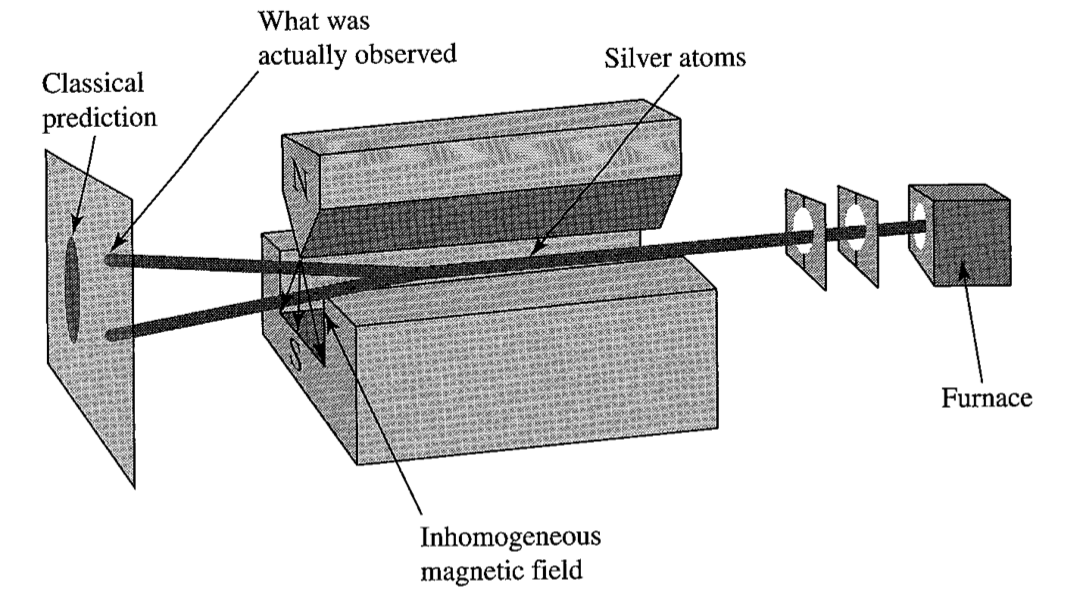
\includegraphics[width = 8cm]{./Sakurai/Fig_1.1.png}
\caption{斯特恩-盖拉赫实验}
\label {Fig1.1}
\end{centering}
\end{figure}

\noindent 我们现在展开一个对斯特恩-盖拉赫实验的简短的讨论 - 这几乎在任何一本现代物理的书中都会被提到\footnote{原注:一个基本但是很有启发性的有关这个实验的讨论请看:French, Anthony Philip, and Edwin F. Taylor. An introduction to quantum physics. CRC Press, 1979. 的第432-438页。\\ 译者注:以及,虽然很不齿,但是最直接的观看相关内容的办法是在新浪爱问里面搜索相关内容。 }。首先,我们先把银原子(Ag)在“烤箱”里面进行加热。这个烤箱呢,在壁上有一个洞;这就导致了一些银原子会从这个洞里面跑出去。如图1.1所示,这些原子,经过一个准直仪后会形成“一束”银原子,然后通过一个由一对有着尖锐边缘的磁铁\footnote{译者注:这里面之所以要用这么复杂的句子来说明这个磁铁,是因为这样才会形成明显的不均匀的磁场。详情可以参考类似于尖端放电等事情。}产生的不均匀的磁场。

我们得研究一下这期间磁场对原子的作用。为此,我们接下来将会极度的简化这个模型。银原子由原子核和47个电子构成,其中的46个原子都可以看成是“隐形的”,它们形成球对称分布从而不对角动量或者其他量产生贡献\footnote{译者注:也就是说,他们都不是最外层电子,由于一些更为复杂的效应,他们在我们的模型里面不贡献。为便于理解,你可以把它想象成一个原子核质量很大的氢原子}。如果我们忽略那个与我们问题不相关的核的自选,我们可以发现,整个原子自身确实有一个仅依赖于电子自旋的角动量 -- 它是一个内禀的量,不像轨道角动量那样 -- 由银原子第47个(5s)电子提供的角动量。第47好电子被束缚在相当于它重量$2\times 10^5$倍的核的附近;因此,这个重原子整体表现了一个与47号电子自旋磁矩相同的磁矩。

\begin{equation}
{\bm{\mu}} \propto S
\end{equation}

\noindent 其中这个准确的比例系数应该是$e/m_e c$\footnote{原注:在本书中$e$<0},精确度大概到了$0.2\%$的量级。

因为磁矩和外磁场的相互作用能是$\boldmath{\mu \cdot B}$,原子在$z$方向上受到的外力是

\begin{equation}
F_z = \frac{\partial}{\partial z}\left(\bm{ \mu \cdot B} \right) \simeq \mu_z \frac{\partial B_z}{\partial z}
\end{equation}

\noindent 其中我们忽略了$\bm{B}$在其它方向上的分量。因为原子整体十分的沉重,我们期望经典意义的“轨道”还能够合理的用到这上面来;至于用海森堡不确定关系处理的办法后面会说到。如图{\ref{Fig1.1}}所示的仪器摆放,$\mu_z > 0\ \left(S_z < 0\right)$的原子受到向下的力,$\mu_z < 0\ \left(S_z > 0\right)$的原子受到向上的力。于是原子束就应该根据$\mu_z$的大小分裂。换句话说,SG(斯特恩-盖拉赫)装置“测量”了$\bm \mu$的$z$分量,也就是说测量了一个正比于$\bm S$的$z$分量的量。

原子在高温箱内排列方向是随机的;它们的$\bm \mu$没有特别偏好的方向。如果电子就像一个经典的在自转的东西,我们可以期待$\mu_z$取从$\left|\bm \mu \right|$ 到$-\left|\bm \mu \right|$的所有值。这使得我们期望看到一摞连续的光束从SG装置内出来。就像{\ref{Fig1.1}}里面那样或多或少的成对称分布在期望的区间内。但是相反的是,我们实际上观察到的,同样是{\ref{Fig1.1}}所展现的,两个特别的“点”被观察到了,伴随着两个自旋的取向——“上”和“下”。换句话说,SG装置把原本的银原子束劈成两个截然不同的成分,这种现象在早期的量子理论中被称为“空间的量子化”。考虑到磁矩$\bm \mu$正比于电子自旋角动量$\bm S$,$S_z$只有两个可能的值:$S_z$向上和$S_z$向下,我们称之为$S_z+$ 和 $S_z-$。这两个可能的$S_z$取值是一些基本的角动量单位的倍数。数字上的来说发现$S_z = \hbar / 2$ 和 $-\hbar / 2$,其中

\begin{equation}
\begin{split}
\hbar & = 1.054 \times 10^{-27} \text{erg-s}\\
& = 6.5822 \times 10^{-16}\text{eV-s}
\end{split}
\end{equation}

\begin{figure}
\begin{centering}
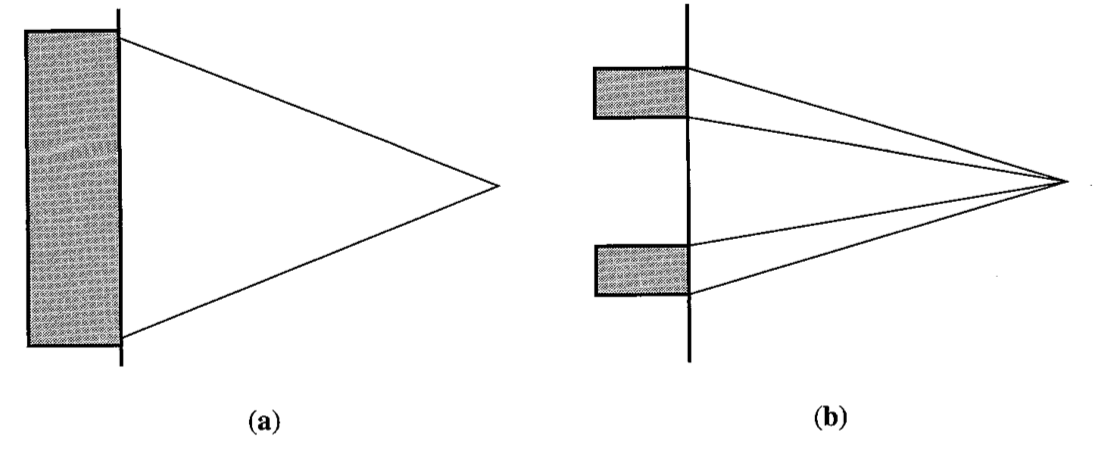
\includegraphics[width = 8cm]{./Sakurai/Fig_1.2.png}
\caption{(a)经典物理预言的斯特恩-盖拉赫实验结果。原子束应该在竖直方向上展开,大小应为磁矩乘以磁矩与竖直夹角的余弦值。然而,斯特恩和盖拉赫观察得到的却是(b),只有两个特定的磁矩方向显现了出来。这两个方向并没有充满在整个预期的范围。}
\label {Fig1.2}
\end{centering}
\end{figure}

\noindent 这个电子自旋角动量“量子化”的现象\footnote{原注:对于如何理解这种量子化的实质,可以参看相对论对量子力学的运用,可以参考本书第8章第2 节的内容。}是我们从斯特恩盖-拉赫实验推得的第一个重要的现象。

图{\ref{Fig1.2}}a 展现了人们预期从实验中观察到的现象;根据经典物理,原子束由于磁矩取向的连续性,自身应该在竖直方向上扩展。但相反的是,人们观察到的是图{\ref{Fig1.2}}b,完全与经典物理相悖。这束光神奇的自己分裂成两束,力部分对应自旋向上,另一部分对应自旋向下。

当然,这种$z$方向的上-下取向并没有什么好惊奇的。我们可以同样将不均匀的场附加在$x$方向让原子束沿$y$方向传播。在这种情况下我们的原子束就会分成$S_x+$成分和$S_x-$成分了。\\

\noindent {\textbf{“并联”的斯特恩-盖拉赫实验}}

\noindent 我们现在考虑一系列“并联”的斯特恩-盖拉赫实验。这是指原子束连续经过两个或更多的SG设备。我们安排了多种方式,第一种是相对直观的一种。我们把从“烤箱”出来的原子束按照图{\ref{Fig1.3}}a中那样依次经过各装置,其中,SG${\hat{\bm z}}$指的是不均匀的磁场在$z$方向。我们如图一样挡住经过第一个SG 装置出来的那些$S_z-$的成分,然后让那些$S_z+$的成分再通过一个其它的SG${\hat{\bm z}}$装置。这一次只有一束出射的原子束 -- 只有$S_z+$成分。这个应该没什么好惊讶的,毕竟如果本身自旋就向上的话,两个SG$\hat{\bm z}$装置之间的几乎可以认为没有的外场不太可能让自旋翻转,所以原子们的自旋应该仍然保持向上。

\begin{figure}
\begin{centering}
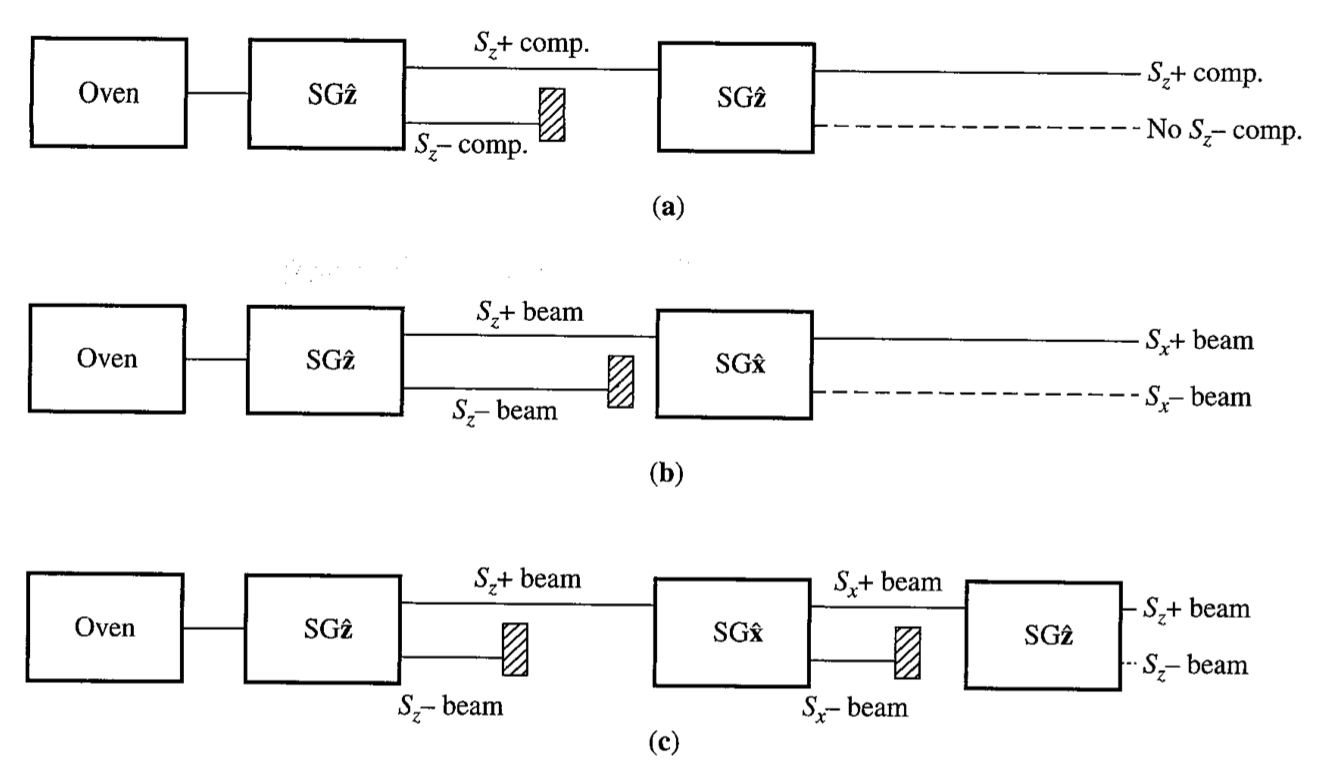
\includegraphics[width = 10cm]{./Sakurai/Fig_1.3.png}
\caption{“并联”的斯特恩-盖拉赫实验(们)}
\label {Fig1.3}
\end{centering}
\end{figure}

令人感兴趣的是图{\ref{Fig1.3}}b中的那种排列方式。在这里,第一个SG装置就像以前一样,但是第二个装置(SG$\hat{\bm x}$)却是在$x$方向上加了不均匀磁场。$S_z+$原子束进入第二个装置(SG$\hat{\bm x}$)现在分裂成两个成分,一个$S_x+$成分,一个$S_x-$成分,都有着同样的强度。我们如何解释这个现象呢?这是不是说$S_z+$原子束中$50\%$的原子是同时具有着$S_z+$和$S_x+$的,同时另外有$50\%$的原子是同时具有着$S_z+$和$S_x-$的呢?这表明这样一幅物理图景面临着很多困难,我们下面会看到。

我们现在考虑第三种玩儿法,如图\ref{Fig1.3}c所示排列。这一步很可能最大程度的展现了量子系统的神奇的地方。这次我们在图{\ref{Fig1.3}}b后面再加入了一个装置,仍然是SG$\hat{\bm z}$类型。我们实验上观察到在第三个新加的装置后面出射了{\textbf{两}}种成分,而不是一种;出射原子束又有$S_z+$成分,又有$S_z-$成分。这实在是令人震惊了,因为从第一个装置出来之后应该就再也没有$S_z-$的成分了。我们想法中一开始就被消除的$S_z-$成分是怎么可能再生的呢?不过显然,原来设想的进入第三个装置的原子束是同时具有$S_z+$和$S_x+$显然并不能产生说服力。

这个例子常常被用来说明量子力学里面我们不能同时的确定$S_z$和$S_x$。更准确的,我们可以说第二个装置(SG$\hat{\bm x}$)做的那个选择完全的破坏了之前的$S_z$ 的信息。

如果把这个情况和一个经典物理里面的旋转的陀螺进行对比会很有趣的。陀螺的角动量为

\begin{equation}
\bm L = I\omega
\end{equation}

\noindent 可以通过测量角速度矢量$\bm \omega$的三个分量来逐一测量。通过观察这个物体转的,和它朝哪个方向转,我们就可以确定$\omega_x, \omega_y, \omega_z$。如果我们知道质量的密度和自转陀螺的几何形状的话,我们就可以得出转动惯量$I$,所以看起来在经典体系下我们可以轻松地区分$L_z$和$L_x$。

可以很直接的感受到,我们遇到的$S_z$和$S_x$不能同时确定的限制并不是由于实验技术的不高超 -- 我们不可能凭借提升实验技术来做到图{\ref{Fig1.3}}c的装置后端不出射原子束。量子力学的特殊性和怪异性被实验本身很好地呈现出来了。而这种(不能同时确定)的限制,事实上,是这个微观现象所固有的。

\noindent {\textbf{与偏振光的类比}}

\begin{figure}
\begin{centering}
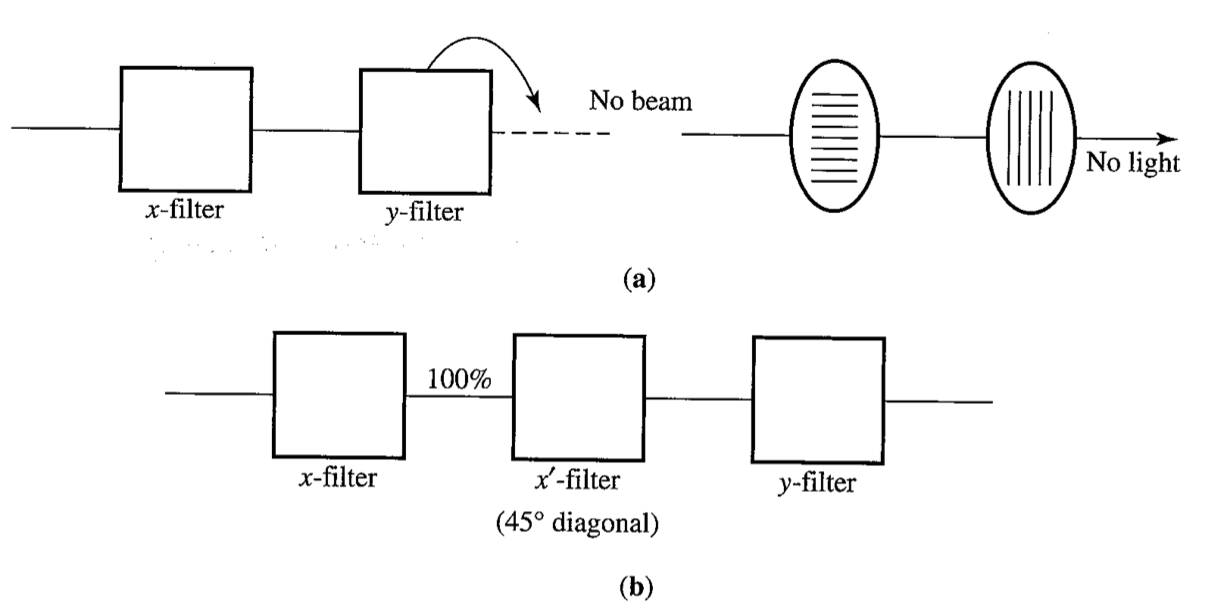
\includegraphics[width = 9cm]{./Sakurai/Fig_1.4.png}
\caption{光束透过偏振片}
\label {Fig1.4}
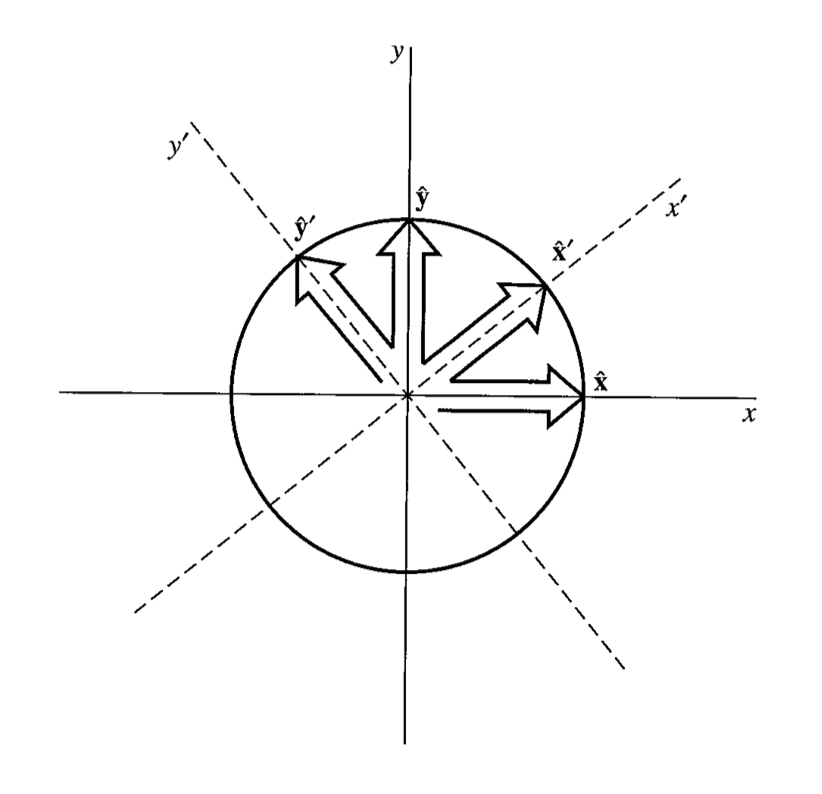
\includegraphics[width = 6cm]{./Sakurai/Fig_1.5.png}
\caption{$x'$和$y'$方向}
\label {Fig1.5}
\end{centering}
\end{figure}

\noindent 因为,自旋的这一套看起来是这么的玄幻,因而做一些与我们已经熟悉的(或是说,经典的)物理体系的类比,对我们理解这套是很必要的。因此,我们先暂时结束讨论,转而看看光波的偏振。这种类比将会帮助我们建立一套针对我们之前做出的量子力学的假定的数学框架。

考虑一束单色光,沿着$z$方向传播。一个线偏振(或平面偏振)的光振动方向在$x$方向。我们简称为$x$偏振光。它应该有如下的电场的时空关系:

\begin{equation} \label{1.1.5}
\bm E = E_0 \hat{\bm x} \cos (kz - \omega t)
\end{equation}

\noindent 同样的,我们考虑一束$y$偏振光,同样沿$z$传播。

\begin{equation} \label{1.1.6}
\bm E = E_0 \hat{\bm y} \cos (kz - \omega t)
\end{equation}

\noindent 有(\ref{1.1.5})或(\ref{1.1.6})形式的偏振光束可以通过让一个未偏振的光通过偏振片来得到。其中,如果某个偏振片只允许$x$方向偏振的光传播的话,那么这个偏振片就被称为$x$偏振片。一个$x$偏振片绕着$z$轴转$90^{\circ}$,理所当然的,就是$y$偏振片了。众所周知,当我们让一束光通过$x$偏振片之后立刻再通过$y$偏振片,那么没有光线会出射出来(假设我们考虑的是理想偏振片);如图\ref{Fig1.4}a。

如果我们在两个偏振片之间再加入一个$x'$偏振片 -- 在$xy$平面上与$x$轴成$45^{\circ}$夹角,如图\ref{Fig1.4}b所示。这回,有一定量的光经过$y$偏振片出来,尽管刚刚出了$x$偏振片之后光束是没有$y$方向电场分量的。换句话说,一旦$x'$介入进来了,并且选择了$x'$方向片真的光束的话,它之前是否是$x$方向不重要。对$x'$方向偏振的筛选破坏了之前光的偏振的一切信息。注意到这个情形和我们之前如图{\ref{Fig1.3}}处理多个SG装置组合是很相似的,就像这样:

\begin{equation} \label{1.1.7}
\begin{split}
S_z \pm \text{原子} \leftrightarrow x-,\ y-\text{偏振光}\\
S_x \pm \text{原子} \leftrightarrow x'-,\ y'-\text{偏振光}
\end{split}
\end{equation}

\noindent 其中,$x'$轴和$y'$轴如图{\ref{Fig1.5}}定义。

我们现在来看看如何在经典电动力学的框架下量化描述一个$45^{\circ}$偏振光($x'$和$y'$轴偏振光)的行为的。由图{\ref{Fig1.5}}我们有

\begin{equation} \label{1.1.8}
\begin{split}
E_0\bm{\hat{x}}'\cos(kz-\omega t) = E_0\left[\frac{1}{\sqrt{2}}\bm{\hat{x}}\cos(kz-\omega t) + \frac{1}{\sqrt{2}}\bm{\hat{y}}\cos(kz-\omega t)\right]\\
E_0\bm{\hat{y}}'\cos(kz-\omega t) = E_0\left[-\frac{1}{\sqrt{2}}\bm{\hat{x}}\cos(kz-\omega t) + \frac{1}{\sqrt{2}}\bm{\hat{y}}\cos(kz-\omega t)\right]
\end{split}
\end{equation}

在图(\ref{Fig1.4})b的三偏振片组合中,原子束从第一个偏振片出来之后是标准的$\hat{\bm x}$偏振。当然也可以这种偏振模式写成$x'$和$y'$偏振的线性叠加,第二个偏振片选择了$x'$偏振的光,同样也可以重新写为$x$和$y$偏振的线性叠加。最后,第三个偏振片选择了$y$偏振的光。

利用(\ref{1.1.7})展现的关系,带入到从图{\ref{Fig1.3}}c的连续斯特恩-盖拉赫实验到图{\ref{Fig1.4}}b的三偏振片实验,我们或许可以把银原子的自旋态用一种新的抽象的二维矢量空间,而不是通常意义的二维($xy$)空间,来表示出来。就如(\ref{1.1.8})中的用$\hat{x}$和$\hat{y}$作为基矢来分解$\hat{x}'$和$\hat{y}'$方向的偏振光,我们同样有道理去把$S_x +$的态用一个矢量来表示 -- 我们把它叫做狄拉克符号中的右矢,下一章我们会详尽的讲狄拉克符号。我们用$\left|S_x ;+\right\rangle$来表示这个矢量,然后把它用另外两个矢量$\left|S_z ;+\right\rangle$,$\left|S_x ;-\right\rangle$(分别代表$z$方向自旋向上\&向下的态)的线性组合。因此,我们推测:

\begin{subequations} \label{1.1.9}
\begin{align}
\left|S_x ;+\right\rangle \overset{?}= \frac{1}{\sqrt{2}} \left|S_z ;+\right\rangle + \frac{1}{\sqrt{2}}\left|S_z ;-\right\rangle \label{1.1.9a}\\
\left|S_x ;-\right\rangle \overset{?}= -\frac{1}{\sqrt{2}}\left|S_z ;+\right\rangle + \frac{1}{\sqrt{2}}\left|S_z ;-\right\rangle
\end{align}
\end{subequations}

\noindent 来类比(\ref{1.1.8})。稍后我们会如何用量子力学的一般方法来得到这些表达式。

总之,那些图(\ref{Fig1.3})c中没被第二个装置(SG$\hat{x}$)挡住的成分,可以看做$S_z +$和$S_z -$的叠加态,就像(\ref{1.1.9a})那样。正因为如此,通过第三个装置(SG$\hat{z}$)后才会有两种成分。

我们紧接着就想到下一个问题:如何确定$S_y \pm$态?对称性说明,如果我们观测到了一个沿着$x$方向传播的$S_z \pm$经过一个SG$\hat{y}$得到的结果应该和观测一个沿着$y$方向传播的$S_z \pm$经过一个SG$\hat{x}$得到的结果非常相似。因此,$S_y \pm$的右矢们当然也应该是$\left|S_z; \pm\right\rangle$的线性叠加啦。但是,从(\ref{1.1.9})中看出,我们似乎已经用尽了所有的组合办法来写$\left|S_x ;\pm\right\rangle$,我们该如何构建矢量空间使得$S_y \pm$态和$S_x$态截然区分呢?

此时,与偏振光的类比再一次拯救了我们。这次我们考虑一束圆偏振光。这可以通过让一束线偏振光穿过四分之一波片来得到。我们让这个圆偏振光通过$x$或$y$偏振片,我们得到$x$方向或$y$方向偏振的光,当然强度是一样的。但是我们当然都知道,这和$45^{\circ}$偏振光($x'$或$y'$偏振)完全不是一回事。

数学上讲,我们如何描述一个圆偏振光呢?右旋圆偏振光无非就是$x$和$y$方向的偏振光的线性组合,其中电场的$y$分量相比于$x$分量有$90^{\circ}$的相位落后\footnote{原注:遗憾的是,左旋和右旋的定义在不同的书中是不一样的}:

\begin{equation}
\bm E = E_0 \left[\frac{1}{\sqrt{2}} \hat{\bm x}\cos\left(kz - \omega t\right) + \frac{1}{\sqrt{2}} \hat{\bm y}\cos\left(kz - \omega t + \frac{\pi}{2}\right)  \right]
\end{equation}

\noindent 一个看起来更精巧的做法是引入复数标记$\epsilon$如下

\begin{equation}
\text{Re}(\epsilon) = \bm{E} / E_0
\end{equation}

\noindent 对于一个右旋偏振光,我们有

\begin{equation}  \label{1.1.12}
\epsilon = \left[\frac{1}{\sqrt{2}} \hat{\bm x}e^{i(kz - \omega t)} + \frac{i}{\sqrt{2}} \hat{\bm y}e^{i(kz - \omega t)}  \right]
\end{equation}

\noindent 其中利用了$i = e^i\pi / 2$

我们可以做如下一个银原子自旋态的类比:

\begin{equation}
\begin{split}
S_y + \text{原子} \leftrightarrow \text{右旋偏振光}\\
S_y - \text{原子} \leftrightarrow \text{左旋偏振光}
\end{split}
\end{equation}

\noindent 把这个类比带入到(\ref{1.1.12})中,我们来看看是否能够把展开的系数补上复数。我们发现把$S_y \pm$原子纳入我们的矢量空间没有任何问题。

\begin{equation}
\left|S_y ;\pm \right\rangle \overset{?}= \frac{1}{\sqrt{2}}\left|S_z ;+\right\rangle \pm \frac{i}{\sqrt{2}}\left|S_z ;-\right\rangle
\end{equation}

\noindent 很明显看起来与(\ref{1.1.9})不一样。于是我们看出来,需要去完整描述银原子自旋的二维矢量空间必须是\emph{复数}空间。任意的一个矢量都会写成$\left|S_z; \pm\right\rangle$的线性组合,当然,一般来讲系数都是复系数。作为一个事实,这么基本的一个例子也明显的需要引入复系数,这还是蛮值得注意的。

读者肯定注意到我们这里故意的避开了光子。换句话说,我们在这里完全没有管光的量子性:我们根本没有提及单光子的偏振态。我们做的类比是描述单一原子的自旋的抽象向量空间中的一个矢量,与\emph{经典电磁场}的偏振矢量的。事实上,我们如果引入光子并讨论一个线偏振态测得圆偏振光的概率或反过来,这会使得这个类比变得更生动;但是,我们并不需要这样。不这么做,我们已经建立了这一节的主要目标:引入量子态的想法,并用复向量空间中的矢量把它表示出来\footnote{原注:对通过光子的偏振来分析的量子力学基本概念这一问题感兴趣的读者,可以参看Baym(1969)的那个很富有启发性的书的第一章。}。

\begin{figure}
\begin{centering}
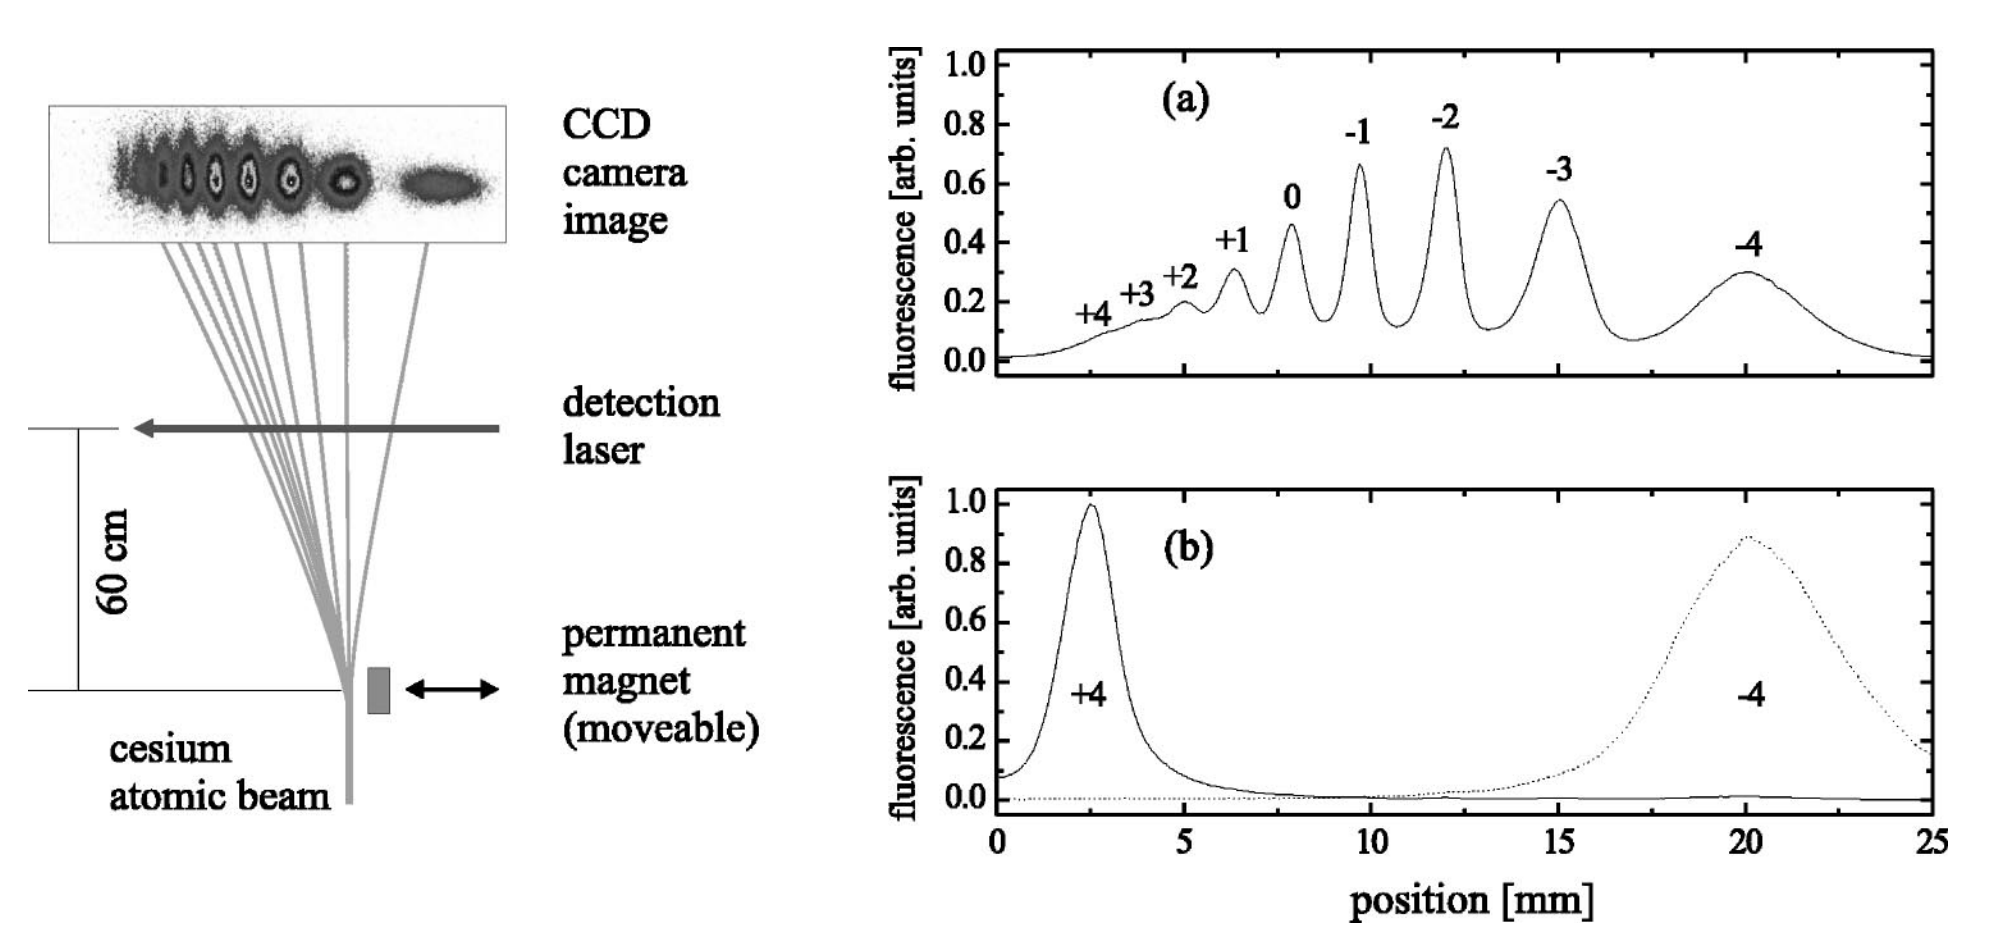
\includegraphics[width = 12.4cm]{./Sakurai/Fig_1.6.png}
\caption{一个现今的斯特恩-盖拉赫实验装置,用来分开原子铯的不同自旋态,图来自F. Lison et al., {\emph {Phys. Rev. A}} {\textbf{61}}(1999) 013405。 装置如左侧显示,数据展现了自旋为4粒子的九个峰,(a)和(b)分别代表筛选最强自旋之前和之后的数据。自旋量子数$F=4$是由于最外层电子的自旋与核自旋$I=7/2$耦合的结果。}
\label {Fig1.6}
\end{centering}
\end{figure}

最终,在给出我们量子力学所需要的数学体系之前,我们着重的强调了斯特恩-盖拉赫装置所展现出来的物理规律,不仅仅是出于对学术的兴趣;分离原子不同的自旋态的能力同样也是我们极为感兴趣的。图{\ref{Fig1.6}}展现了用斯特恩-盖拉赫技术分析了对铯原子束自旋进行操作的结果。这个碱金属它唯一稳定的同位素,$\ ^{133}\text{Cs}$,的核自旋$I = 7/2$,而实验发现粒子束分成了$9$个自旋取向的$F = 4$超精细磁态。这仅仅是诸多把这一一度神秘的现象用于实际装置的例子之一罢了。当然啦,这么多的实验更加的使我们确信了我们接下来要展现并讨论的量子力学基本原理。


\subsection{左矢,右矢和算符}

\noindent 前面的章节我们展现了对斯特恩-盖拉赫实验的分析是如何引导我们去想象一个复数的向量空间的。从这节开始,接下来的章节讲建立一套用于量子力学的基本的向量空间数学形式。我们这本书使用的是P. A. M. Dirac建立的左矢、右矢符号。尽管早在量子力学建立之前线性代数就发展了很久且完善了,Dirac这种引入向量空间的办法仍然有许多优势,尤其是从物理学家的角度来说。

\ 

\noindent \textbf{右矢空间}

\noindent 我们物理里面考虑一个有特定维数的复向量空间。在斯特恩-盖拉赫型的实验里面,这个特定的维数就是由原子的自旋决定的,根据原子经过SG仪之后分裂成的路线得到。在银原子里面,就是$2$,因为只有两种$S_z$\footnote{尽管很多物理系统的维度实际上是不可数无穷多的,我们这里通常仍然会使用一个有限的数$N$来表示,因为绝大多数情况下结论对不可数无穷多也是适用的。}。在后面,节\ref{s1.6}中,我们会考虑连续谱,比如坐标本征态活着动量本征态,这时候维数是不可数无穷多的,这时候这种向量空间只能被称为\emph{Hilbert空间}\footnote{D. Hilbert研究了无穷维度的向量空间,里面有一些问题和有限维是不一样的}。

在量子力学中,一个物理态,比如说一个有确定自旋方向的银原子,由一个复向量空间中的{\emph{态矢量}}来描述。我们管这样一个矢量叫做“右矢”,并且用$|\alpha\rangle$来标记他。在这套理论中,这样一个右矢包含了这个物理态的完整的信息,所有关于这个物理态我们能够了解的信息都可以通过态矢量获得。两个态矢量也可以相加:

\begin{align}
|\alpha\rangle + |\beta\rangle = |\gamma\rangle
\end{align}

\noindent 加出来的结果$|\gamma\rangle$就是另一个不同的态矢量了。如果我们给$|\alpha\rangle$乘上一个任意的复数$c$,得到的结果$c|\alpha\rangle$也是另一个态矢量。这个数$c$是写在态矢量的左边和右边没有什么区别

\begin{align}
c|\alpha\rangle = |\alpha\rangle c
\end{align}

\noindent 特别的,当$c=0$的时候,得到的右矢是一个{\emph{空右矢}}。

一个基于物理的假设是,当$c\neq 0$的时候,$|\alpha\rangle$和$c|\alpha\rangle$代表着相同的物理态,换句话说,只有在向量空间中的“方向”才是重要的。数学家们可能更倾向于说我们处理的是“射线”而不是矢量。

一个{\emph{客观测量}},比如说动量,自旋分量,可以由一个作用在我们这里的向量空间中的{\emph{算符}}来描述,比如$A$。一般的,算符作用在右矢的左边。

\begin{align}
A\cdot(|\alpha\rangle) = A|\alpha\rangle
\end{align}

\noindent 得到另一个向量。后面我们会更多的讨论这种乘上去的算符。

一般的,$A|\alpha\rangle$并不会得到一个常数乘以$|\alpha\rangle$。然而,一些特殊的也是重要的右矢,我们称为算符$A$的{\emph{本征态}},

\begin{align}
|a’\rangle,|a’’\rangle,|a’’’\rangle,\cdots
\end{align}

\noindent 它们满足

\begin{align}\label{1.2.5}
A|a’\rangle = a’|a’\rangle,A|a’’\rangle = a’’|a’’\rangle,\cdots
\end{align}

其中,在态矢量外边的那些$a’, a’’,\cdots$都只是数。注意,将$A$作用在这样一个本征矢量上仅仅得到一个数乘以这个本征态矢。这些数组成的集合$\{a’,a’’,a’’’,\cdots\}$,或者用$\{a’\}$来指代,被称为算符$A$的本征值。当必要时可以用排好序的本征值序列$\{a^{(1)},a^{(2)},a^{(3)},\cdots\}$来代替原本的$\{a’,a’’,a’’’,\cdots\}$。

由本征态矢描述的物理态被称为{\emph{本征态}}。在最简单的自旋$\frac{1}{2}$体系中,\eqref{1.2.5}表示的本征值-本征态矢之间的关系就是

\begin{align}
S_z|S_z;+\rangle = \frac{\hbar}{2}|S_z;+\rangle,\quad S_z|S_z;-\rangle = -\frac{\hbar}{2}|S_z;-\rangle
\end{align}

其中$|S_z;\pm\rangle$是算符$S_z$的本征态矢,本征值分别为$\pm\hbar/2$。因此我们可以用$|\hbar/2\rangle$来指代$|S_z;+\rangle$,与我们之前的符号$|a'\rangle$是一致的——用本征值来标记本征态矢。不过鉴于我们前面已经非常熟悉$|S_z;\pm\rangle$这套符号了,我们这里出于方便的角度继续使用,而且这样一来表述$S_x$的本征态矢也就很清晰简单了:

\begin{align}
S_x|S_x;\pm\rangle = \pm\frac{\hbar}{2}|S_x;\pm\rangle
\end{align}

我们之前注意到向量空间的维度是由施特恩-盖拉赫型实验的出射结果的数量决定的。更严格的来说,我们考虑一个$N$-维的向量空间有$N$个算符$A$的本征矢来展开。任意一个右矢可以写成

\begin{align}
|\alpha\rangle = \sum_{a'}c_{a'}|a'\rangle
\end{align}

\noindent 其中$a', a'', \cdots$直到$a^{(N)}$,其中$c_{a'}$是一个复的系数。这样展开的唯一性的证明我们后面会在讲本征态矢的正交性的时候讲。

\ 

\noindent {\textbf{左矢空间和内积}}

\noindent 至今为止我们处理的向量空间都是右矢的向量空间,现在我们引入{\emph{左矢空间}}的概念——这是一个与右矢空间“对偶”的空间。我们假设对于每一个右矢$|\alpha\rangle$,在对欧空间(即左矢空间)中存在一个左矢,用$\langle \alpha|$标记。左矢空间可以用本征左矢$\{\langle a'|\}$来展开,每一个这里面的本征左矢都和右矢空间中的本征态矢对应$\{|a'\rangle\}$,这是一个一对一的对应关系:

\begin{equation}
\begin{split}
|\alpha\rangle &\overset{\text{DC}}{\longleftrightarrow}\langle\alpha|\\
|a'\rangle, |a''\rangle, \cdots&\overset{\text{DC}}{\longleftrightarrow}\langle a'|,\langle a''|,\cdots\\
|\alpha\rangle + |\beta\rangle &\overset{\text{DC}}{\longleftrightarrow} \langle\alpha|+\langle\beta|,
\end{split}
\end{equation}

\noindent 其中DC表示\emph{对偶对应}。粗略地讲,我们可以把左矢空间看成右矢空间的某种镜像。

左矢空间中,与$c|\alpha\rangle$对偶的是$c^*\langle\alpha|$,\emph{不是}$c\langle\alpha|$。这是一个很重要的点。一般的,我们有

\begin{align}
c_{\alpha}|\alpha\rangle + c_{\beta}\overset{\text{DC}}{\longleftrightarrow}c_{\alpha}^*\langle\alpha|+c_{\beta}^*\langle\beta|
\end{align}

我们现在定义一个左矢和右矢的内积\footnote{在各种文献中,内积通常指的是\emph{标量积}因为这和欧几里德空间中的$\bf a\cdot b$是类似的;然而在这本书中,我们只管在三维空间中转动下保持不变的量称之为\emph{标量}}。内积写成左矢在左而右矢在右的形式,比如,

\begin{align}
\langle\beta|\alpha\rangle = \underset{\text{bra(c)ket}}{\displaystyle(\langle\beta|)\cdot(|\alpha\rangle)}
\end{align}

这个内积,通常来说,是一个复数。注意到在构造这样一个内积的时候,我们总是从bra空间和ket空间各取一个矢量。

我们假设两个关于内积的基本性质,首先

\begin{align}\label{1.2.12}
\langle\beta|\alpha\rangle = \langle\alpha|\beta\rangle^*
\end{align}

\noindent 换句话说,$\langle\beta|\alpha\rangle$和$\langle\alpha|\beta\rangle$彼此是复共轭。注意尽管某种程度上,这个内积和我们熟悉的标量积$\bf a\cdot b$很像,$\langle\beta|\alpha\rangle$必须与$\langle\alpha|\beta\rangle$严格的区分开来,而矢量空间的$\bf a\cdot b = b\cdot a$。利用\eqref{1.2.12},我们可以立刻得到$\langle\alpha|\alpha\rangle$必然是一个实数。证明只需要让$\langle\beta|\to\langle\alpha|$

第二个内积的假设是

\begin{align}
\langle\alpha|\alpha\rangle\ge0
\end{align}

\noindent 其中等号仅在$|\alpha\rangle$是{\emph{零矢量}}的时候才成立。有些文献中这条假设也被称为{\bf{正定矩阵}}。从物理学家的角度来看,这条假设实际上是量子力学的概率诠释的本质,我们后面会看到这一点\footnote{一些吧这条假设抛弃的尝试导致``非正定矩阵''的物理理论的出现;我们这本书里面不会讲这点。}。

两个ket$|\alpha\rangle,|\beta\rangle$如果满足下面的条件我们就把它俩定义为正交的:

\begin{align}\label{1.2.14}
\langle\alpha|\beta\rangle = 0
\end{align}

\noindent 尽管在内积的定义中是$\langle\alpha|$这种以bra出现的形式。正交关系\eqref{1.2.14}通过\eqref{1.2.12}同样说明:

\begin{align}
\langle\beta|\alpha\rangle = 0
\end{align}

给出一个不是零矢量的ket,我们可以构造一个{\bf 归一化矢量}$|\tilde{\alpha}\rangle$,其中

\begin{align}
|\tilde{\alpha}\rangle = \left(\frac{1}{\sqrt{\langle\alpha|\alpha\rangle}}\right)|\alpha\rangle
\end{align}

\noindent 满足性质

\begin{align}\label{1.2.17}
\langle\tilde{\alpha}|\tilde{\alpha}\rangle = 1
\end{align}

\noindent 一般的,$\sqrt{\langle\alpha|\alpha\rangle}$被称为$|\alpha\rangle$的{\bf 模},类似于三位欧几里得矢量里面的$\sqrt{\bf a\cdot a} = |\bf a|$。因为$|\alpha\rangle$与$c|\alpha\rangle$表达了相同的物理态,我们通常也会要求我们使用的物理态是如同\eqref{1.2.17}\footnote{对于连续谱的本征态又不一样的归一化要求,我们会在节\ref{s1.6}中见到。}一样归一化的。

\ 

\noindent {\bf{算符}}

\noindent 我们之前说过,可观测量(比如动量,自旋的分量)可以通过作用在ket上的算符来描述。我们可以考虑更为普遍的作用在ket上的算符,$X, Y$等等,而$A,B$仍然只带那些代表可观测量的算符。

算符作用在右矢(ket)的左边

\begin{align}
X\cdot(|\alpha\rangle)=X|\alpha\rangle
\end{align}

\noindent 得到的结果是另一个ket。算符$X, Y$被定义成{\bf 相等}

\begin{align}
X=Y
\end{align}

\noindent 如果对于{\emph{任意的}}在考虑的体系下ket空间中的ket,

\begin{align}
X|\alpha\rangle = Y|\alpha\rangle
\end{align}

\noindent 算符$X$如果对于任意的ket$|\alpha\rangle$都满足下列性质的话则被称为{\bf 零算符}:

\begin{align}
X|\alpha\rangle = 0
\end{align}

\noindent 算符满足叠加性,其加法有交换律和结合律
\setcounter{equation}{20}
\begin{subequations}
\begin{align}
X+Y=&Y+X\\
X+(Y+Z)=&(X+Y)+Z
\end{align}
\end{subequations}

\noindent 除了章{\ref{Ch4}}中考虑的时间反演对称算符,我们这本书的算符都是线性的;也就是说

\begin{align}
X(c_\alpha|\alpha\rangle+c_\beta|\beta\rangle)=c_\alpha X|\alpha\rangle + c_\beta X|\beta\rangle
\end{align}

算符$X$作用在左矢bra的右边

\begin{align}
(\langle\alpha|)\cdot X=\langle\alpha|X
\end{align}

\noindent 然后得到另一个左矢。右矢$X|\alpha\rangle$和左矢$\langle\alpha|X$,普遍的讲,与彼此并不是对偶的。我们定义一个符号$X^\dagger$:

\begin{align}\label{1.2.24}
X|\alpha\rangle\overset{\text{DC}}{\longleftrightarrow}\langle\alpha|X^\dagger
\end{align}

\noindent 算符$X^\dagger$被称为$X$的Hermitian伴算符,或者简称伴算符。算符$X$被称为Hermitian算符如果

\begin{align}
X=X^\dagger
\end{align}

\ 

\noindent {\bf{乘积}}

\noindent 算符$X, Y$可以相乘。算符的乘积一般来说是{\emph{不可交换的}},也就是说

\begin{align}
XY\neq YX
\end{align}

\noindent 而另一方面,算符的乘积是可以结合的

\begin{align}\label{1.2.27}
X(YZ)=(XY)Z=XYZ
\end{align}

\noindent 我们同样有

\begin{align}
X(Y|\alpha\rangle) = (XY)|\alpha\rangle = XY|\alpha\rangle,\quad (\langle\beta|X)Y=\langle\beta|(XY)=\langle\beta|XY
\end{align}

\noindent 注意到

\begin{align}
(XY)^\dagger=Y^\dagger X^\dagger
\end{align}

\noindent 因为

\begin{align}
XY|\alpha\rangle = X(Y|\alpha\rangle)\overset{\text{DC}}{\longleftrightarrow}(\langle\alpha||Y^\dagger)X^\dagger = \langle\alpha|Y^\dagger X^\dagger
\end{align}

到现在为止,我们考虑了如下这些``积'':$\langle\beta|\alpha\rangle,X|\alpha\rangle,\langle\alpha|X,XY$。是否还有一些其他的技我么能弄呢?让我们试试把$|\beta\rangle$和$\langle\alpha|$,按照另一重顺序乘起来,得到

\begin{align}
(|\beta\rangle)\cdot(\langle\alpha|)=|\beta\rangle\langle\alpha|
\end{align}

\noindent 被称为$|\beta\rangle$和$\langle\alpha|$的{\bf 外积}。我们会在后面强调$|\beta\rangle\langle\alpha$也要被考虑成一个算符;因此它与内积(一个数)是有着本质的区别的。

当然,也存在着一些``不合法的积''。我们提到过算符必须作用在ket的左边,bra的右边换句话说,$|\alpha\rangle X, X\langle\alpha|$都是不合法的积。它们既不是ket,也不是bra,也不是算符;它们压根没有意义。形如$|\alpha\rangle|\beta\rangle,\langle\alpha|\langle\beta|$的积当$|\alpha\rangle$和$|\beta\rangle$(或者其相应的对偶)是在相同的ket(bra)空间中的时候,也是不合法的。\footnote{在本书的后面中,我们会遇到形如$|\alpha\rangle|\beta\rangle$的形式,或者更准确的写成$|\alpha\rangle\otimes|\beta\rangle$,但是这些情况下$|\alpha\rangle$和$|\beta\rangle$知道的是{\emph{不同}}矢量空间的。比如说,第一个ket属于电子自旋的矢量空间,而第二个ket属于电子轨道角动量;或者第一个ket属于第一个粒子,第二个ket属于第二个例子,或者其他类似这样的。}

\ 

\noindent {\bf{结合律公理}}

\noindent 从\eqref{1.2.27}中,我们能清楚地看到算符的成绩是具有结合律的。事实上,这种结合律的性质是我们为了普遍的处理``合法''的态而做的对左矢、右矢以及算符进行的假定。Dirac管这个重要的假定称作{\bf 乘法结合律公理}。

我们首先考虑如下的外积作用在一个右矢上,从而看看这条公理的强大之处:

\begin{align}\label{1.2.32}
(|\beta\rangle\langle\alpha|)\cdot|\gamma\rangle
\end{align}
因为结合律公理,我们可以把它等价的写成

\begin{align}\label{1.2.33}
|\beta\rangle\cdot(\langle\alpha|\gamma\rangle)
\end{align}

\noindent 其中,$\langle\alpha|\gamma\rangle$仅仅是一个数。这样的话,外积作用在右矢上就得到了另一个右矢。另一方面,$|\beta\rangle\langle\alpha|$也可以看做是一个算符。由于\eqref{1.2.32}和{1.2.33}实际上是完全一样的,我们可以略去那个乘号把它写作$|\beta\rangle\langle\alpha|\gamma\rangle$来代表算符$\beta\rangle\langle\alpha|$作用在$\gamma$上,{\it 或者},可以看成是数$\langle\alpha|\gamma\rangle$乘以$|\beta\rangle$。(另一方面,如果\eqref{1.2.33}写成$(\langle\alpha|\gamma\rangle)\cdot|\beta\rangle$,我们并不能略去那个乘号和括号,因为它导致的结果很可能看起来不太合法。)注意到算符$|\beta\rangle\langle\alpha|$作用在$|\gamma\rangle$上使得它``转动''的朝向$|\beta\rangle$方向。可以很直观的看到,如果
\be
X=|\beta\rangle\langle\alpha|
\ee
那么,
\be
X^\dagger = |\alpha\rangle\langle\beta|
\ee
其证明留做练习。

另一个有关结合律公理的重要的示例是
\be\label{1.2.36}
(\underset{\text{左矢}}{\langle\beta|})\cdot(\underset{\text{右矢}}{X|\alpha\rangle}) = (\underset{\text{左矢}}{\langle\beta|X})\cdot(\underset{\text{右矢}}{|\alpha\rangle})
\ee
因为这两边是相等的,我们就可以进而使用一个更简介的符号
\be
\langle|X|\alpha\rangle
\ee
来表示\eqref{1.2.36}的两边。我们之前讲过左矢$\langle\alpha|X^\dagger$和右矢$X|\alpha\rangle$是对偶的,于是我们可以写
\be\label{1.2.38}
\begin{split}
\langle\beta|X|\alpha\rangle& = \langle\beta|\cdot(X|\alpha\rangle)\\
&=\{(\langle|X^\dagger)\cdot|\beta\rangle\}^*\\
&=\langle\alpha|X^\dagger|\beta\rangle^*
\end{split}
\ee
其中,除了结合律公理之外,我们用了内积的基本性质\eqref{1.2.12}。对于一个{\it Hermitian}的算符$X$,我们有
\be
\langle\beta|X|\alpha\rangle = \langle\alpha|X|\beta\rangle^*
\ee



\subsection{基矢和算符的矩阵表示}

\noindent {\bf{可观测量的本征态}}

\noindent 让我们考虑Hermitian算符$A$的本征态和本征值。我们用$A$这个记号来表示我们之前的可观测量,因为在量子力学里面,Hermitian算符通常来说会代表物理中的可观测量。

我们首先陈述一个定理

\begin{theo}
Hermitian算符$A$的本征值是实的;它的对应不同本征值的本征态彼此正交。
\end{theo}

\noindent {\emph{证明}}. 首先,我们记得
\be\label{1.3.1}
A|a'\rangle = a'|a'\rangle
\ee
因为$A$是Hermitian的,我们同样有
\be\label{1.3.2}
\langle a''|A = a''^*\langle a''|
\ee
其中$a',a'',\cdots$是$A$的本征值。如果我们在\eqref{1.3.1}的两边同时在左边作用一个$\langle a''|$上去,并且在\eqref{1.3.2}两边右边同时作用一个$|a'\rangle$上去,并且相减,我们有
\be\label{1.3.3}
(a'-a''^*)\langle a''|a'\rangle = 0
\ee
而这里$a'$和$a''$可以是相同或者不同的。首先我们把它们取成相同的,我们得到了对本征值为实数的要求(也就是定理的前半部分)
\be
a' = a'^*
\ee
其中我们使用了条件:$|a'\rangle$不是一个空态矢。我们现在假定$a'$和$a''$不在一致。利用我们刚刚证明的定理的前半部分,在\eqref{1.3.3}中的$a'-a''^*=a'-a''$,根据我们的假设,它并不得$0$。因此内积必须得$0$:
\be
\langle a''|a'\rangle = 0,\quad (a' \neq a'')
\ee
保证了正交性(定理的第二部分)。\ \\

我们希望我们的物理体系中的可观测量具有实的本征值在下一节我们讨论测量在量子力学中的描述的时候可能看的更清楚。我们刚刚证明的定理确保当算符是Hermitian的时候其本征值就是实数。这就是我们如此强调量子力学中的Hermitian可观测量的原因。

一般来讲,我们会去吧$|a'\rangle$归一化得到正交归一(orthonormal)的集$\{|a'\rangle\}$:
\be\label{1.3.6}
\langle a''|a'\rangle = \delta_{a''a'}
\ee
我们当然可能会去问,这套本征态是否完备呢?因为我们在最开始的讨论的时候假定整个右矢空间是用$A$的本征态展开的,所以通常来讲$A$的本征右矢必须是完备的从而能{\it 构建}我们的右矢空间\footnote{原注:敏锐的读者如果已经对波动力学熟悉的话可疑之处本征函数的完备性可以用对Schrodinger方程是用Sturm-Liouville(斯图姆-刘伟尔)理论。但是从我们的基本假设出发来``得到''Schrodinger方程的过程中,位置本征态的完备性必须被假定。}。\\

\noindent {\bf{本征右矢作为右矢基矢}}

\noindent 我们看到$A$的归一本征态构成了完备正交归一集合。右矢空间的任意一个右矢可以用$A$的本征右矢展开;换句话说,$A$的本征右矢可以用来作为右矢基矢,就像欧几里得(Euclidean)空间里面的彼此正交的单位矢量作为基矢一样。

给定一个右矢$|\alpha\rangle$,可以按照如下方式用$A$的本征右矢展开:
\be\label{1.3.7}
|\alpha\rangle = \sum_{a'}c_{a'}|a'\rangle
\ee
左乘一个$\langle a''|$并且利用正交归一条件\eqref{1.3.6},我们得到展开系数
\be
c_{a'} = \langle a'|\alpha\rangle
\ee
换句话说,我们有
\be\label{1.3.9}
|\alpha\rangle = \sum_{a'}|a'\rangle\langle a'|\alpha\rangle
\ee
类似于在Euclidean空间里面一个(实的)矢量$\bf V$进行展开:
\be
{\bf V} = \sum_i\hat{\bf e}_i(\hat{\bf e}_i\cdot\bf V)
\ee
其中$\{\hat{\bf e}_i\}$构成了正交的单位矢量。我们现在回忆乘法的结合律公理:$|a'\rangle\langle a'|\alpha\rangle$可以视为数$\langle a'|\alpha\rangle$乘以$|a'\rangle$或者,相等的,算符$|a'\rangle\langle a'|$作用在$|\alpha\rangle$上。由于\eqref{1.3.9}是任意一个矢量,我们必须有
\be\label{1.3.11}
\sum_{a'}|a'\rangle\langle a'| = 1
\ee
其中等式右边的$1$可以理解为一个单位算符,\eqref{1.3.11}被称为{\bf 完备性关系},或者{\bf 闭包}(closure)。

\eqref{1.3.11}的有用性永远不会被高估。如果给定右矢,算符或者左矢作用在合法的顺序时,我们可以在任何我们觉得方便的位置插入如\eqref{1.3.11}那样的单位算符。比如,我们考虑计算$\langle\alpha|\alpha\rangle$;在$\langle\alpha|$和$|\alpha\rangle$中间插入单位算符,我们有
\be
\begin{split}
\langle\alpha|\alpha\rangle&=\langle\alpha|\cdot\left(\sum_{a'}|a'\rangle\langle a'|\right)\cdot|\alpha\rangle\\
&=\sum_{a'}|\langle a'|\alpha\rangle|^2
\end{split}
\ee
这个恰好说明了,如果$|\alpha\rangle$是归一化的,那么\eqref{1.3.7}中的展开系数必然满足
\be
\sum_{a'}|c_{a'}|^2 = \sum_{a'}|\langle a'|\alpha\rangle|^2 = 1
\ee

我们现在来看看\eqref{1.3.11}中的$|a'\rangle\langle a'|$。因为这是一个外积,其也必然是一个算符。将其作用在$|\alpha\rangle$上:
\be
(|a'\rangle\langle a'|)\cdot|\alpha\rangle = |a'\rangle\langle a'|\alpha\rangle = c_{a'}|a'\rangle
\ee
我们看到$|a'\rangle\langle a'|$挑选出了$|\alpha\rangle$中平行于$|a'\rangle$的部分,所以$|a'\rangle\langle a'|$就被成为了沿着右矢$|a'\rangle$的{\bf 投影算符},记为$\Lambda_{a'}$
\be
\Lambda_{a'}\equiv|a'\rangle\langle a'|
\ee
完备性关系\eqref{1.3.11}现在就可以写为
\be
\sum_{a'}\Lambda_{a'}=1
\ee
\ \\

\noindent {{\bf 矩阵表示}}

\noindent 当我们选定一组右矢基矢之后,就可以按照下面的方法用一个方阵,$X$,来表示我们的算符了。首先,利用\eqref{1.3.11}两次,我们可以把算符$X$写成
\be
X = \sum_{a''}\sum_{a'}|a''\rangle\langle a''|X|a'\rangle\langle a'|
\ee
总共有$N^2$个形如$\langle a''|X|a'\rangle$的数,其中$N$是右矢空间的维数。我们可以把它排列成一个$N\times N$的矩阵形式,行和列如下所示
\be
\langle \underset{\text{行}}{a''}|X|\underset{\text{列}}{a'}\rangle
\ee
每项都写出来的话我们有
\be
X \overset{\cdot}{=}\left(\begin{matrix}
\langle a^{(1)}|X|a^{(1)}\rangle & \langle a^{(1)}|X|a^{(2)}\rangle & \cdots\\
\langle a^{(1)}|X|a^{(1)}\rangle & \langle a^{(1)}|X|a^{(1)}\rangle & \cdots\\
\vdots & \vdots & \ddots \end{matrix}\right)
\ee
其中符号$\overset{\cdot}{=}$表示``被表示为''\footnote{原注:我们这里不使用等号是因为矩阵的表示取决于特定的基矢选取。算符与算符的表示是两个不同的概念,就像演员与演员的海报的关系。}

用\eqref{1.2.38},我们可以写出
\be
\langle a''|X|a'\rangle = \langle a'|X^\dagger|a''\rangle^*
\ee
而如\eqref{1.2.24}定义的Hermitian伴算符与{\it 共轭转置}这个或许大家更熟悉的概念联系起来。如果算符$B$是Hermitian的,我们有
\be
\langle a''|B|a'\rangle = \langle a'|B|a''\rangle^*
\ee

我们把$\langle a''|X|a'\rangle$写成矩阵的形式是与矩阵的乘法规则相一致的。只要注意到算符矩阵表示的关系(如下)就能看到这点:
\be
Z = XY
\ee
也就是
\be\begin{split}
\langle a''|Z|a'\rangle &= \langle a''|XY|a'\rangle\\
&=\sum_{a'''}\langle a''|X|a'''\rangle\langle a'''|Y|a'\rangle
\end{split}\ee
我们只是再一次的插入了单位算符\eqref{1.3.11}在$X, Y$之间!

我们现在检验右矢关系
\be
|\gamma\rangle = X|\alpha\rangle
\ee
是否能被我们的基矢来表示。展开系数可以通过左乘一个$\langle a'|$得到:
\be\begin{split}
\langle a'|\gamma\rangle &= \langle a'|X|\alpha\rangle\\
&=\sum_{a''} \langle a'|X|a''\rangle\langle a''|\alpha\rangle
\end{split}\ee
但是这可以看做方阵乘法规则作用在列矢量上的一个应用,只要我们把$|\alpha\rangle$和$|\gamma\rangle$摆成列矢量的样子:
\be
|\alpha\rangle \overset{\cdot}{=} \left(\begin{matrix}
\langle a^{(1)}|\alpha\rangle\\
\langle a^{(2)}|\alpha\rangle\\
\langle a^{(3)}|\alpha\rangle\\
\vdots
\end{matrix}\right),\quad |\gamma\rangle \overset{\cdot}{=}\left(\begin{matrix}
\langle a^{(1)}|\gamma\rangle\\
\langle a^{(2)}|\gamma\rangle\\
\langle a^{(3)}|\gamma\rangle\\
\vdots
\end{matrix}\right)
\ee
类似的,如果有
\be
\langle\gamma| = \langle\alpha|X
\ee
我们可以考虑
\be
\langle \gamma|a'\rangle = \sum_{a''}\langle \alpha|a''\rangle\langle a''|X|a'\rangle
\ee
所以一个左矢可以通过行矢量按照如下方式表示:
\be\label{1.3.29}\begin{split}
\langle &\overset{\cdot}{=} (\langle\gamma|a^{(1)}\rangle,\langle\gamma|a^{(2)}\rangle,\langle\gamma|a^{(3)}\rangle,\ldots)\\
&=(\langle a^{(1)}|\gamma\rangle^*,\langle a^{(2)}|\gamma\rangle^*,\langle a^{(3)}|\gamma\rangle^*,\ldots)
\end{split}\ee
注意到写成\eqref{1.3.29}这种行矢量的时候,其行元会有一个复共轭。内积$\langle\beta|\alpha\rangle$可以写成行矢量表示的$\langle\beta|$和列矢量表示的$|\alpha\rangle$的乘积:
\be\begin{split}
\langle\beta|\alpha\rangle &= \sum_{a'}\langle\beta|a'\rangle\langle a'|\alpha\rangle\\
&=(\langle a^{(1)}|\beta\rangle^*,\langle a^{(2)}|\beta\rangle^*,\langle a^{(3)}|\beta\rangle^*,\ldots) \left(\begin{matrix}
\langle a^{(1)}|\alpha\rangle\\
\langle a^{(2)}|\alpha\rangle\\
\langle a^{(3)}|\alpha\rangle\\
\vdots
\end{matrix}\right)
\end{split}\ee
如果我们用行矩阵表示$\langle\alpha|$左乘到$|\beta\rangle$是千年古,我们得到了前面的那个表达式的复共轭,与我们\eqref{1.2.12}的内积基本性质是一致的。

\noindent 最后,外积$|\beta\rangle\langle\alpha|$的矩阵表述可以写为
\be
|\beta\rangle\langle\alpha|\overset{\cdot}{=}\left(\begin{matrix}
\langle a^{(1)}|\beta\rangle\langle a^{(1)}|\alpha\rangle^* & \langle a^{(1)}|\beta\rangle\langle a^{(2)}|\alpha\rangle^* & \ldots\\
\langle a^{(2)}|\beta\rangle\langle a^{(1)}|\alpha\rangle^* & \langle a^{(2)}|\beta\rangle\langle a^{(2)}|\alpha\rangle^* & \ldots\\
\vdots & \vdots & \ddots
\end{matrix}\right)
\ee

可观测量$A$的矩阵表示如果我们使用$A$的本征态的话就会很简单。首先我们有
\be
A = \sum_{a''}\sum_{a'}|a''\rangle\langle a''|A|a'\rangle\langle a'|
\ee
但是我们会发现方阵$\langle a''|A|a'\rangle$显然是对角的:
\be
\langle a''|A|a'\rangle = \langle a'|A|a'\rangle\delta_{a'a''} = a'\delta_{a'a''}
\ee
所以
\be\label{1.3.34}\begin{split}
A&=\sum_{a'}a'|a'\rangle\langle a'|\\
&=\sum_{a'}a'\Lambda_{a'}
\end{split}\ee

\noindent {\bf 自旋$\frac{1}{2}$系统}

现在来考虑一下特殊的自旋$\frac{1}{2}$系统是很有指导意义的。基矢我们选为$|S_z;\pm\rangle$,我们简写为$|\pm\rangle$。在这个空间下最简单的算符就是单位算符,根据\eqref{1.3.11}可以写为
\be
1 = |+\rangle\langle+|+|-\rangle\langle-|
\ee
根据\eqref{1.3.34},我们当然可以把$S_z$写成
\be
S_z = (\hbar/2)[(|+\rangle\langle+|)-(|-\rangle\langle_|)]
\ee
本征右矢关系为
\be
S_z|\pm\rangle = \pm(\hbar/2)|\pm\rangle
\ee
从$|\pm\rangle$的正交归一性中立即得到。

与此同时,另外两个算符也值得我们花时间去研究:
\be
S_+ = \hbar|+\rangle\langle-|,\quad S_- = \hbar|-\rangle\langle+|
\ee
这两个算符都是{\it 非}Hermitian的。算符$S_+$作用在自旋向下态$|-\rangle$会把它变成自旋向上态$|+\rangle$乘以$\hbar$。与此相对,如果是用$S_+$作用在自旋向上态$|+\rangle$上,就会变成空矢量。因此,物理上对这个$S_+$的解释是它可以提升自旋分量一个$\hbar$;如果自旋分量不能再被提升了,我们就得到了一个空态。类似的,$S_-$被解释为使自旋分量降低$\hbar$的算符。后面我们会看到$S_\pm$可以写成$S_x\pm iS_y$。

在构建角动量算符的矩阵表示的时候,




\subsection{测量,可观测量和不确定关系}
\subsection{变换基矢的情况}
\subsection{坐标,动量和平移} \label{s1.6}
\subsection{坐标空间和动量空间的波函数}

\end{document}
